\documentclass[a4paper,10pt,twocolumn,uplatex]{jsarticle}
\usepackage{style/nislab,style/resume}

%---------------------------------------------------------------------
% レジュメ種別・日付設定(要変更)
% \type{} 1:修士論文諮問会 2:卒業論文発表会 else:月例発表会
\type{3}
\year{2021}
\month{10}
\date{9}

%---------------------------------------------------------------------
% ページ番号設定(要変更)
\setcounter{page}{1}

%---------------------------------------------------------------------
\begin{document}
%---------------------------------------------------------------------
% タイトル作成部分(要変更)
% \maketitle{タイトル}{title}{名前}{name}
\maketitle{ARを用いた時空間表現による仮想ドローン操縦手法}
{週}
{竹内 一真}
{Kazuma Takeuchi}

%---------------------------------------------------------------------
\section{はじめに}
近年,ドローンは空中を移動することで高い機動性を発揮し,建築物や社会インフラの点検まで,幅広い分野で活躍できる機器として注目されている.
その中でも,ドローン操縦には自律飛行と遠隔操作の二種類の操縦法が主に使用されている\cite{sample}.
技術の進歩により,自動的に飛行する自律飛行が注目されつつあるが,人間がドローンを操縦する「遠隔操作」では,人間の意図を直接ドローンに反映できる利点があるため,
ドローンを用いて事故を起こすわけにはいかないようなインフラの点検などでは,遠隔操作による操縦が行われている.
\par
このように遠隔操作は自律飛行とは異なり,より緊密に操縦者の操縦意図とドローンの動作を結びつける,細かい作業を行うような場面で利用される.
しかし,遠隔操作には操縦者の技量、や,高い集中力を要するため,ドローンと障害物の距離の推定や,ドローンの向きや姿勢,どのような動きをするかの推定など,
遠隔操作を行いながら他の作業を行うことが困難である\cite{teleoperate}.
\par
そこで,本研究では操縦者が遠隔操作を手軽に行えるような新しいインタフェースを提案する.
具体的には,AR(Augmented Reality)の技術を活用することで,現実のドローンに加えて仮想的なドローンを表示させる.
仮想ドローンと操縦者のインタラクションにより,操縦者の技量や高い集中力を軽減した遠隔操作を提供できるか検討する.
\par

%---------------------------------------------------------------------

\begin{figure}[!tb]
  \centering
  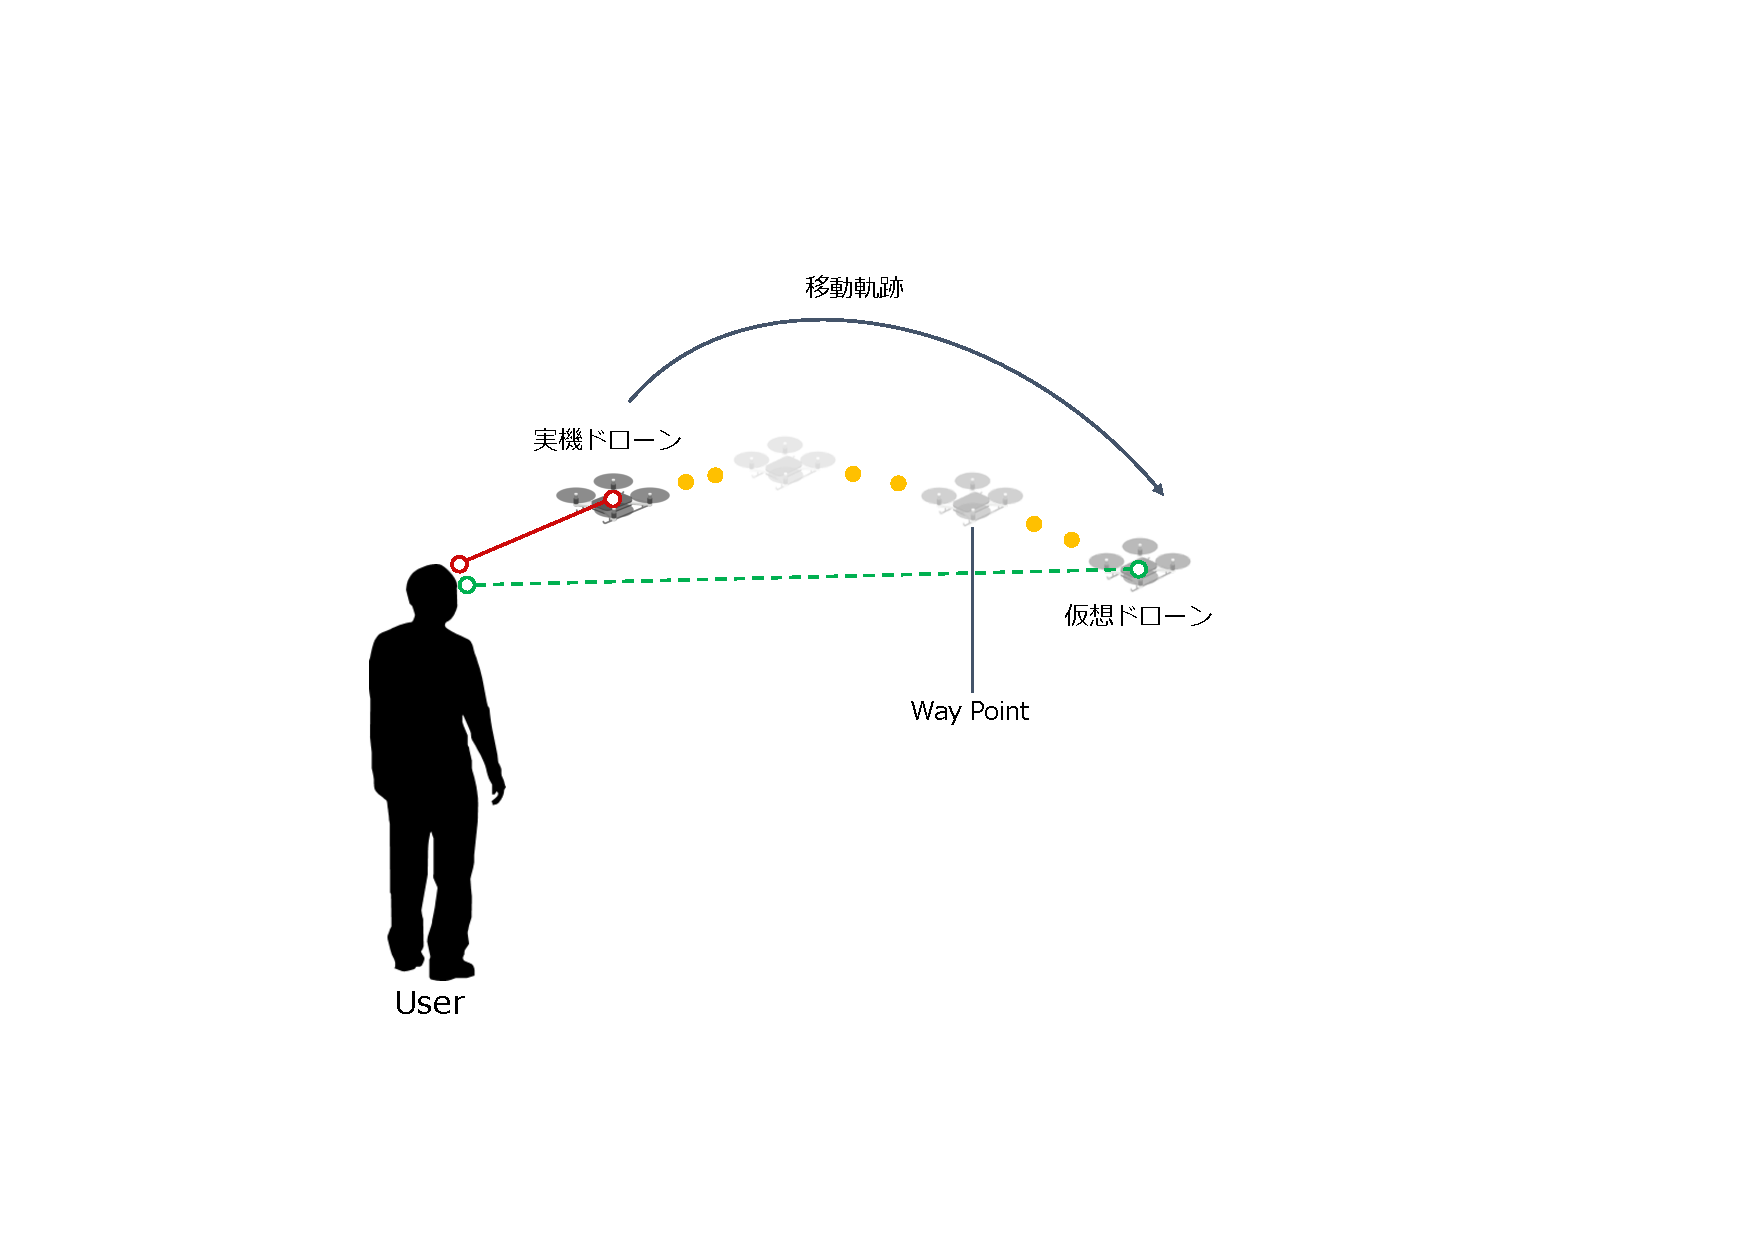
\includegraphics[width=\linewidth]{img/movement.pdf}
  \caption{時空間ドローン操縦のインタフェースデザイン}
  \label{fig:movement}
\end{figure}

%---------------------------------------------------------------------

\section{関連研究}\label{discussion}
Yuanzhiらの研究では,人間とロボットの共同作業(HRC)において音声やジェスチャーを用いたロボットとのコミュニケーションでは非効率性や
曖昧さが生じる可能性があることを問題視している.
そこで,ボディトラッキングを利用してユーザの動きを記録し,ARによりレンダリングして表示し,
ユーザーはその行動を自由に観察,編集,推論することで,ロボットの動作プランを導き出す手法を提案している\cite{time-space}.
結果として,ユーザにリアルタイムで空間的に位置する視覚的なタスクオーサリング能力を提供しながら,
より高いレベルの協調的作業を達成することができた.
人間の体の動きを時空間的に表現することで,ロボットとのインタラクションを図っていたが,ドローンは人間と構造が異なるため,
人間の動きを参考にすることはできない.
しかし,時空間的に表現されたユーザの動きを参考にしながらロボットとのコミュニケーションを行えたことより,時空間表現は有効であると考える.

%---------------------------------------------------------------------

\section{提案手法}\label{discussion}
\subsection{概要}
本研究では,操縦者は直接ドローンを操縦することなく,仮想ドローンを操縦することで,安全な遠隔操作を提供できるか検討する.
仮想ドローンを操縦した際,移動した軌跡をARにより表示することで,実機ドローンが周囲の環境にどのような影響を及ぼすかを予見し,
快適な操縦を提供できると仮説を立てる.


\subsection{時空間ドローン操縦手法}
実際に存在するドローンと,ARにより表示された同じ位置に存在する仮想ドローンを操縦者に提供する.
仮想ドローンを操縦した際には,図\ref{fig:movement}のように移動した各Way Pointに対して仮想ドローンを時空間参照でき,どのように実機のドローンを
移動させるかを確認することができる.また,衝突の恐れがあると判断した際は,Way Pointを戻すことで修正を行う.
実機のドローンは最終的に決定した経路を追いかけるように移動し,仮想ドローンと同じ位置にある際に停止する.

%---------------------------------------------------------------------


\subsection{動作手順}
提案手法の動作手順を図\ref{fig:sequence}に示す.
具体的な流れを以下に示す.
\begin{enumerate}
  \item 仮想ドローンを到達したい地点まで進める
  \item 時空間表示されたWay Pointを参照する
  \item 表示されたままの軌跡で周辺の環境に影響を及ぼさないか判断する
  \item 実機のドローンをその軌道に合わせて自動で追従させる
  \item 仮想ドローンの最終位置まで到達したら停止する
\end{enumerate}

%---------------------------------------------------------------------

\begin{figure}[!tb]
  \centering
  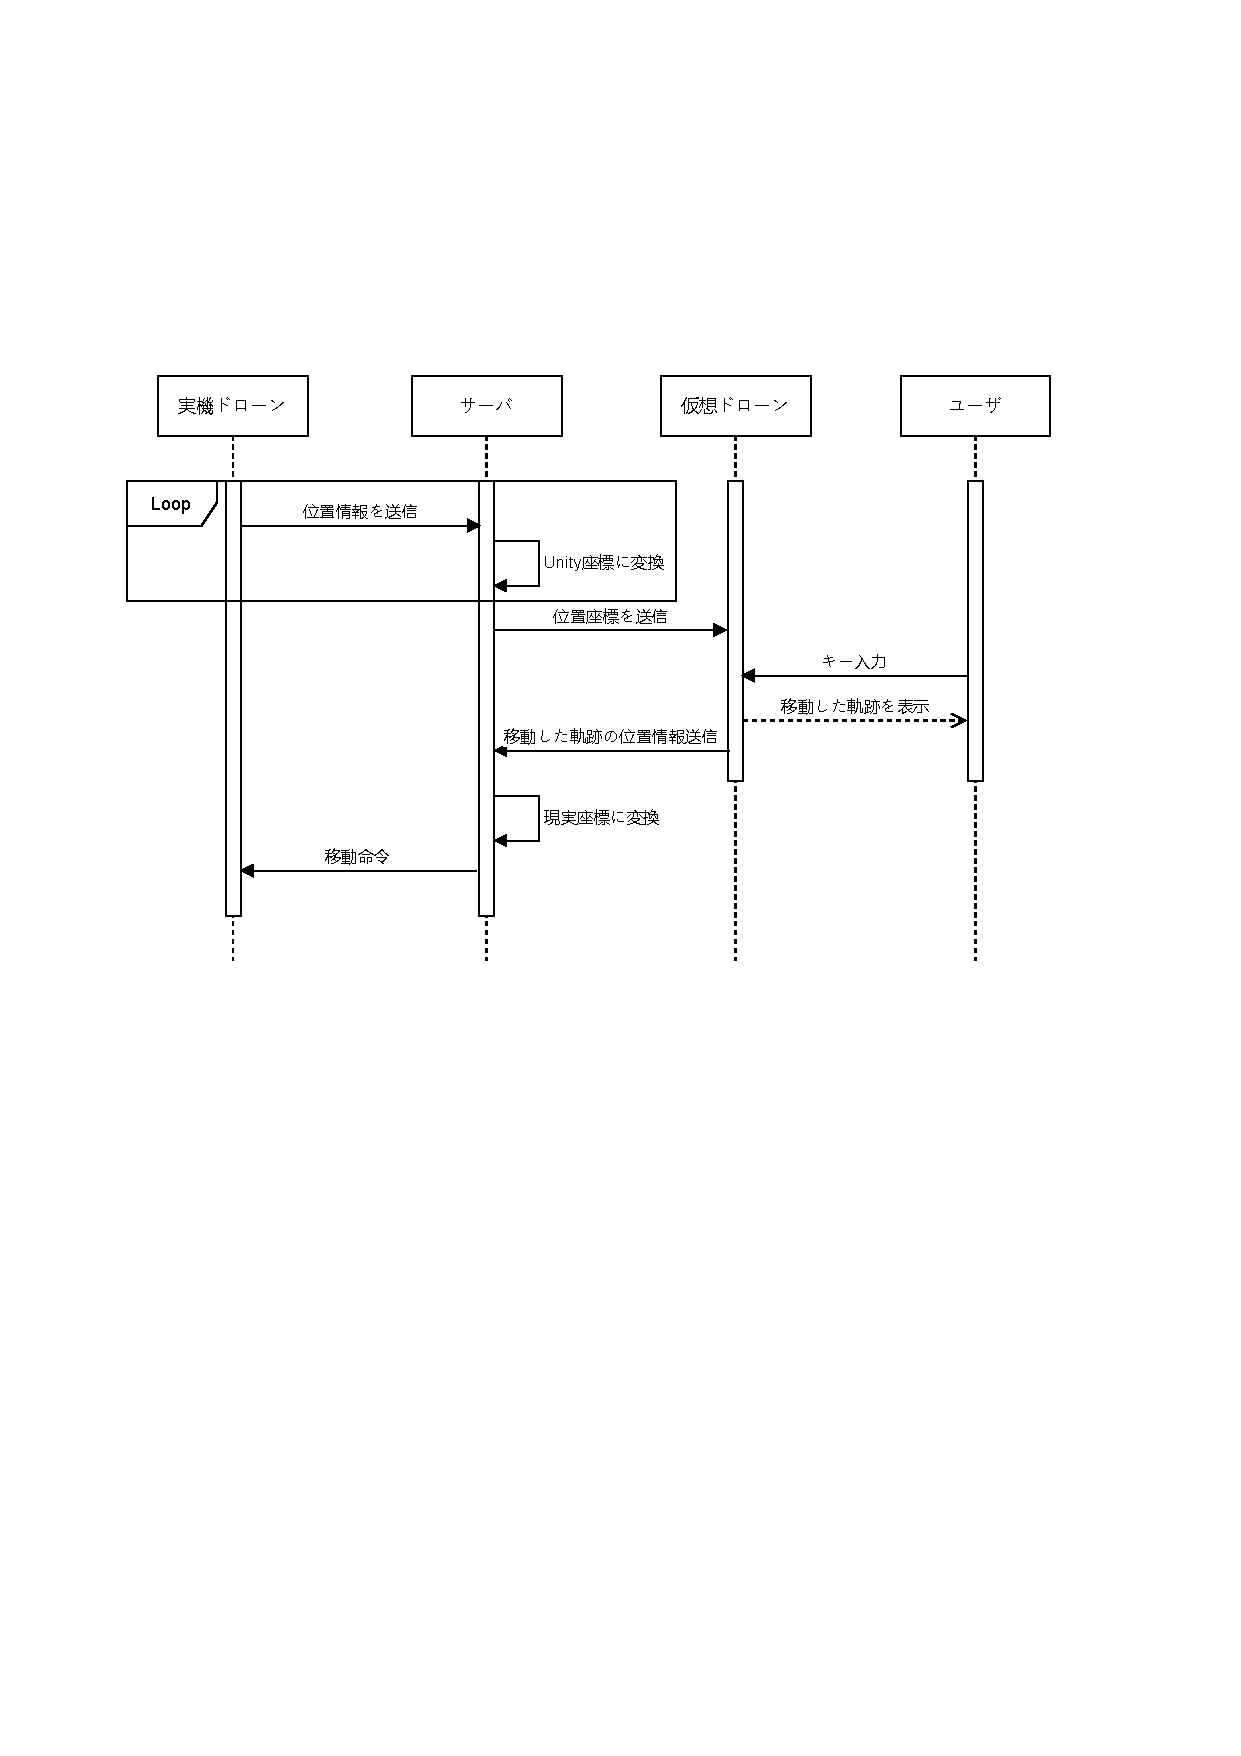
\includegraphics[width=\linewidth]{img/sequence.pdf}
  \caption{提案手法のシーケンス図}
  \label{fig:sequence}
\end{figure}

%---------------------------------------------------------------------

\section{評価}\label{experiment}
\subsection{システム構成}
提案手法のシステム構成を図\ref{fig:overview}に示す.
ドローンはTello EDU,ARHMDはMicrosoft HoloLens2,サーバはMac-BookProを用いる.
システムはHoloLens2上でUnityアプリケーションが動作しており,Unity内で仮想ドローンを配置する.
サーバでは常時Tello EDUの傾きや姿勢,移動距離をHoloLens2に送信する.
サーバでは受け取った値をUnity座標系に変換し,返還後の値を反映させる.
また,コントローラで入力された値を一定期間サーバに保持しておき,実機のドローンを進行させる際にUnity座標系より実世界の座標系に変換し,
実機のドローンを進行させる.


\subsection{実験}
ARなしの従来の操縦,本提案手法を比較することで,ARを用いた手法の有効性を検証する.
実験参加者はドローンをスタート地点から操縦し,目的地点に到着させるタスクを行う.
その間,衝突の恐れのある障害物を設置し,衝突することなく正確に通過することを要求する.
操縦者は近距離までドローンに近づくことなく,遠距離で操縦することとする.


\subsection{評価項目}
本提案手法を用いることによって遠隔操作を手軽に行えるかを検証するため,主観的評価と客観的評価を行う.
主観的評価として使いやすさ,遠距離からの操縦しやすさ,客観的評価として実験参加者がタスクを完了するまでのタスク完了時間を評価する.

%---------------------------------------------------------------------

\begin{figure}[!tb]
  \centering
  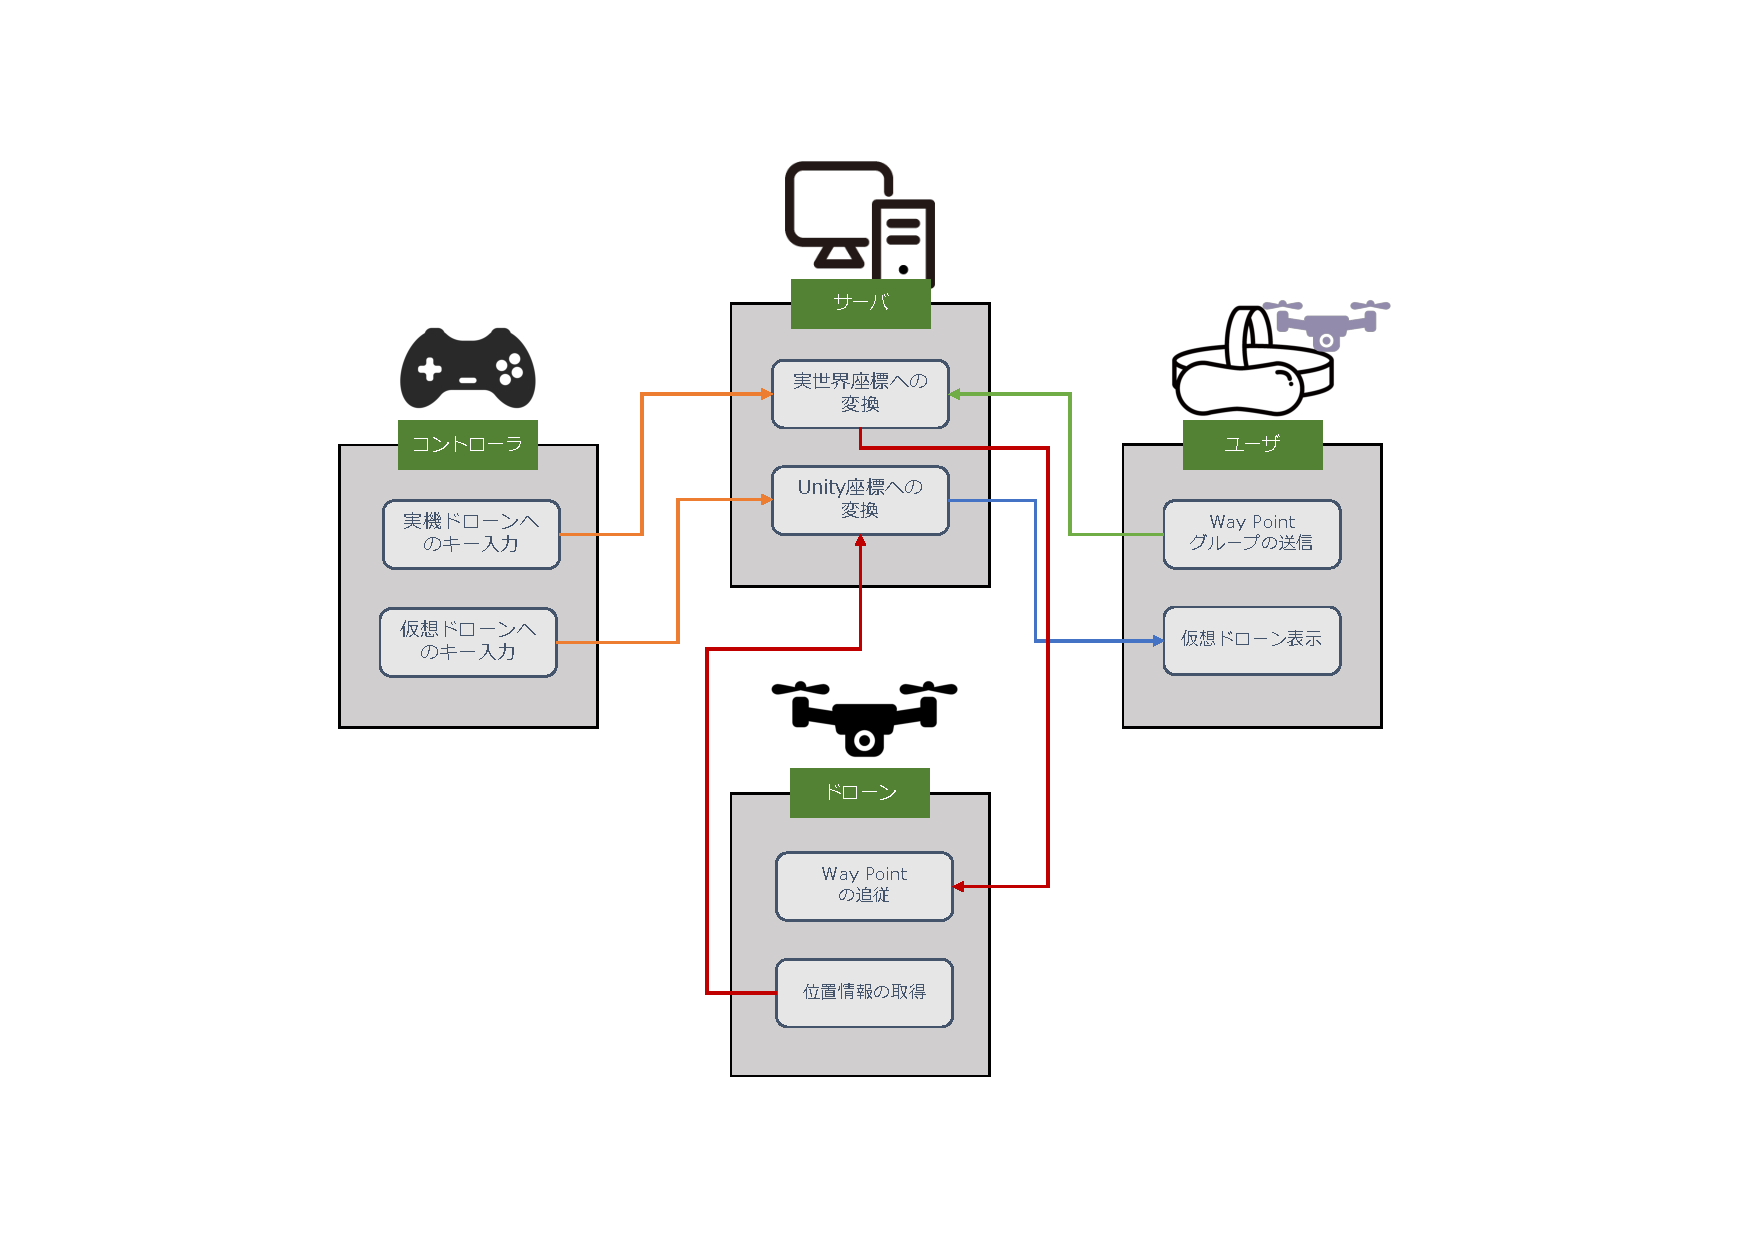
\includegraphics[width=\linewidth]{img/overview.pdf}
  \caption{システム構成}
  \label{fig:overview}
\end{figure}

%---------------------------------------------------------------------
\section{まとめと今後の課題}
遠隔操作によるドローン操縦では,操縦者の技量や,操縦による高い集中力を要するため,遠隔操作を行いながら他の作業を行うことが困難である.
そこで本研究では,操縦者が遠隔操作を手軽に行えるように新しいインタフェースを提案した.
ARの技術を活用することで,現実のドローンに加えて仮想的なドローンを表示させ,仮想ドローンを操縦した際の移動した動きを実機のドローンに
追従させる。
遠隔操作への集中負荷を軽減できるか検証し,提案手法の有用性を示す.
\par
今後の課題は,提案手法における仮想ドローンの配置頻度のパラメータ設定を行う.
また,本提案手法によって遠隔操作が手軽に行えたことを示すため,今後はマルチタスクにも着目した実験シナリオの設定,具体的な評価項目を検討する.

%---------------------------------------------------------------------


% \subsection{表}
% 表は\tabref{tab:data_type}のように引用することができ,表を作成する場合は罫線を少なくすることと,横線のみの使用を心がけることが推奨される.

% \begin{table}[!bt]
%   \caption{代表的なデータの型}
%   \label{tab:data_type}
%   \centering
%   \begin{tabular}{lcr}
%     \hline
%     データの型         & 宣言   & ビット幅 \\
%     \hline \hline
%     短整数型           & short  & 16       \\
%     整数型             & int    & 32       \\
%     単精度浮動小数点型 & float  & 32       \\
%     倍精度浮動小数店型 & double & 64       \\
%     \hline
%   \end{tabular}
% \end{table}

%---------------------------------------------------------------------
% \section{研究者にとっての論文十箇条}
% 論文を書くことは大切だ必要だ,と周囲から言われる.それは自分でも分かっているつもりだけれど,その理由をはっきりと伝えてもらえる機会は少ない.研究者にとっての論文十箇条\cite{whats_paper}は,とてもシンプルでわかりやすく,非常に心にきた.一度目を通してみるべきであろう.

% \begin{enumerate} % 箇条書きは \begin{itemize}
% \item 書かれた論文は書いた人の研究者としての人格を表す
% \item データのみ出して論文を書かない者は,テクニシャンである
% \item データも出さず,論文(原著論文)を書かない者は,評論家である
% \item 研究者は論文を書くことによって成長する.また,成長の糧にしなければならない
% \item 論文は研究者の飯のタネである
% \item 論文は後世の研究に影響を与えなければならない
% \item 研究者は書いた論文に責任を問われる
% \item 忙しくて論文が書けないというのは,言い訳にはならず,能力がないといっているのと同じである
% \item 博士論文以上の論文を書けない者は,その博士論文は指導教官のものといわれても仕方がない
% \item 研究において最も重要なのはアイデアであり,それが試されるのが論文である
% \end{enumerate}

%---------------------------------------------------------------------
% Bibliography
\footnotesize{
  \begin{thebibliography}{99}
    \bibitem{sample} プラントにおけるドローン活用事例集,経済産業省
    \bibitem{teleoperate} J. Y. Chen, E. C. Haas, and M. J. Barnes, “Human Performance Issues
    and User Interface Design for Teleoperated Robots,” IEEE Transactions
    on Systems, Man, and Cybernetics, Part C (Applications and Reviews),
    vol. 37, no. 6, pp. 1231–1245, 2007.
    \bibitem{time-space} Yuanzhi Cao, Tianyi Wang, Xun Qian, Pawan S Rao,
    Manav Wadhawan, Ke Huo, and Karthik Ramani. 2019.
    GhostAR: A Time-space Editor for Embodied
    Authoring of Human-Robot Collaborative Task with
    Augmented Reality. In Proceedings of the 32nd Annual
    ACM Symposium on User Interface Software and
    Technology. 521–534. 
  \end{thebibliography}
}

%---------------------------------------------------------------------
\end{document}
%---------------------------------------------------------------------
